\documentclass[11pt,a4paper]{article}

\usepackage[utf8]{inputenc}
\usepackage[T1]{fontenc}
\usepackage[spanish]{babel}
\usepackage[margin=2cm, bottom=6.2cm, footskip=1.7cm]{geometry}
\usepackage{graphicx}
\graphicspath{{../../01_Propuesta/Logos/}{./}}
\usepackage{fancyhdr}
\usepackage{xcolor}
\usepackage[hidelinks]{hyperref}
\usepackage{enumitem}
\usepackage{array}
\usepackage{needspace}
\setlist{nosep}
\setlength{\parindent}{0pt}
\setlength{\parskip}{8pt}

\definecolor{verdeosc}{RGB}{26,107,60}
\definecolor{verdemid}{RGB}{46,139,87}

\pagestyle{fancy}
\fancyhf{}
\fancyfoot[C]{%
  \noindent{\color{verdeosc}\rule{\textwidth}{0.8pt}}\\[6pt]
  \tiny
  \hyphenpenalty=10000\exhyphenpenalty=10000
  \noindent
  \begin{minipage}{\textwidth}
  \begin{minipage}[t]{4.4cm}
  {\color{verdeosc}\textbf{ORGANIZA}}\\[3pt]
  Grupo de Investigación IN SILICO\\[6pt]
  {\color{verdeosc}\textbf{CO-ORGANIZADORES}}\\[3pt]
  Departamento de Biología y Química\\
  Departamento de Ingeniería Agroindustrial\\
  Departamento de Ingeniería Agrícola\\
  Departamento de Física\\
  Universidad de Sucre
  \end{minipage}%
  \hfill
  \begin{minipage}[t]{3.7cm}
  {\color{verdeosc}\textbf{COORDINACIÓN}}\\[3pt]
  \textbf{Aldo F. Combariza}\\
  Coordinación General\\
  \textbf{María Ximena Díaz}\\
  Coordinación Académica\\
  \textbf{Sebastián Vargas}\\
  Coordinación Logística\\
  \textbf{Selena Arias Avila}\\
  Coordinación Administrativa
  \end{minipage}%
  \hfill
  \begin{minipage}[t]{3.7cm}
  {\color{verdeosc}\textbf{CONTACTO}}\\[3pt]
  \textbf{SICVEC 2026}\\
  19--20 de octubre de 2026\\
  C.C. Guacarí, Sincelejo\\
  Modalidad híbrida\\
  \href{mailto:insilico@unisucre.edu.co}{insilico@unisucre.edu.co}
  \end{minipage}%
  \end{minipage}%
}
\renewcommand{\headrulewidth}{0pt}

\begin{document}

\noindent

\includegraphics[height=1.6cm]{logo_sicvec2026.png}%
\hspace{10pt}{\color{verdeosc}\vrule width 1.2pt height 1.5cm}\hspace{10pt}%
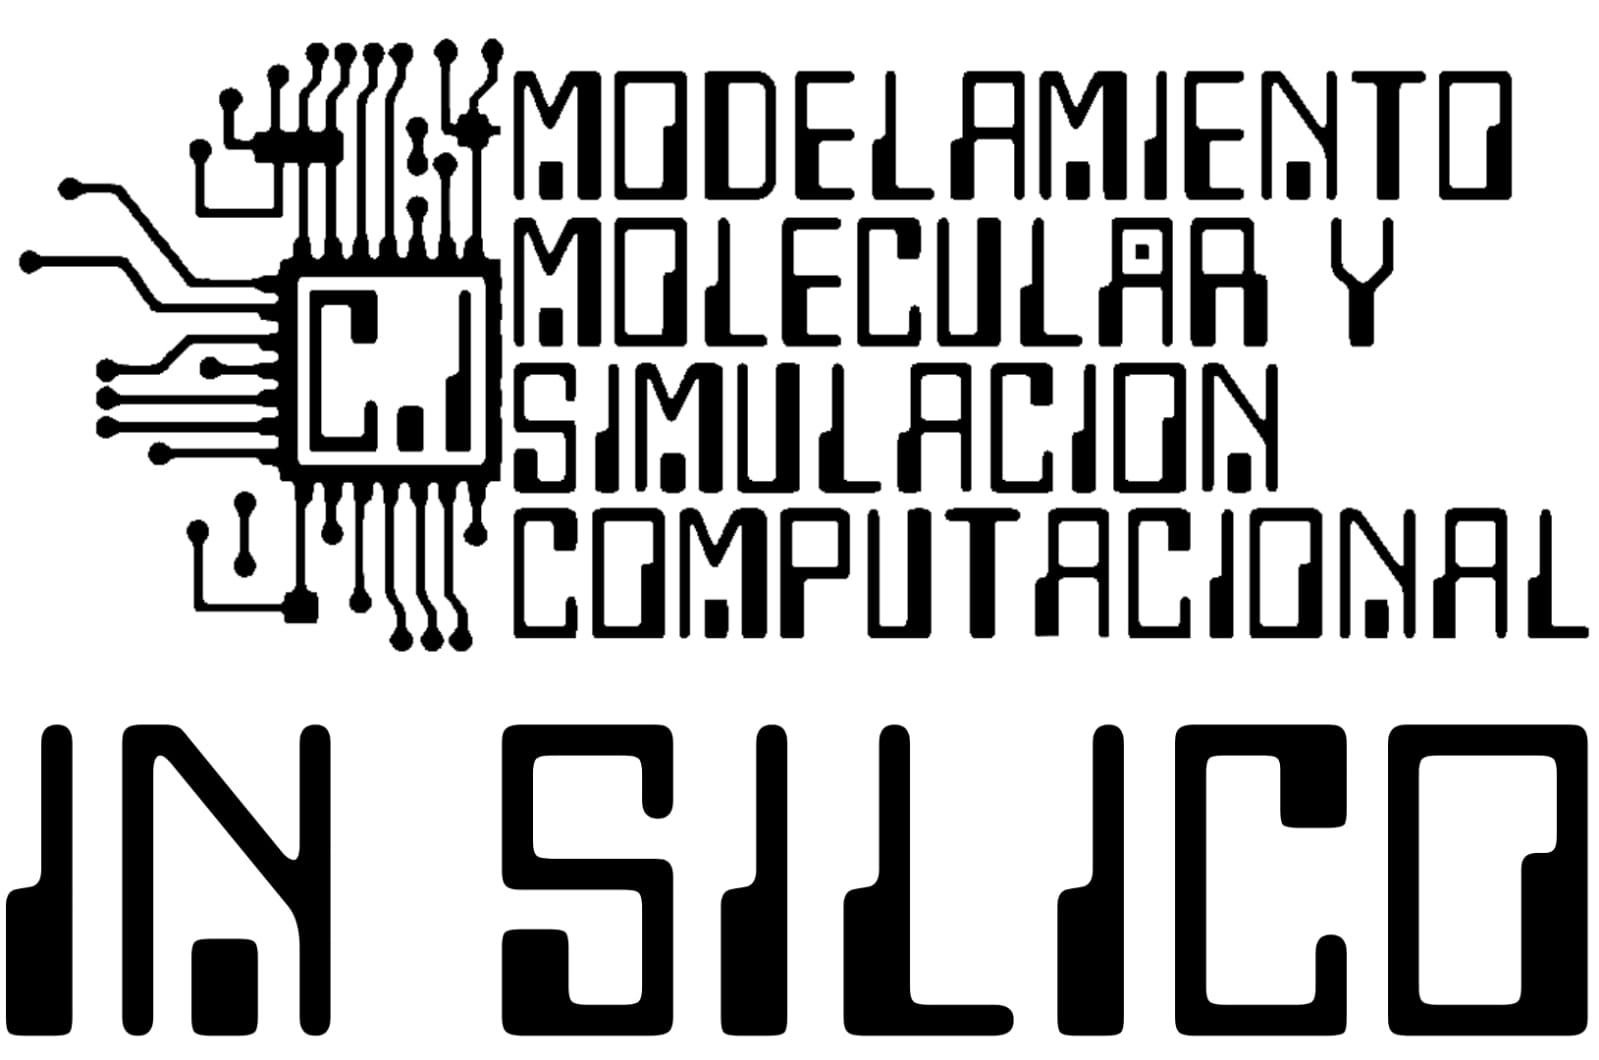
\includegraphics[height=1.28cm]{Logo_insilico.jpeg}%
\hspace{10pt}{\color{verdeosc}\vrule width 1.2pt height 1.5cm}\hspace{10pt}%

\includegraphics[height=1.3cm]{Logo_Bio.png}\hspace{6pt}%

\includegraphics[height=1.3cm]{logo_agroin.png}\hspace{6pt}%

\includegraphics[height=1.3cm]{logo_ingagrocola.png}\hspace{6pt}%

\includegraphics[height=1.3cm]{logo_fisica_lifi.png}%
\hspace{10pt}{\color{verdeosc}\vrule width 1.2pt height 1.5cm}\hspace{10pt}%

\includegraphics[height=1.3cm]{logo_unisucre.png}

\vspace{0.3cm}

\noindent
\textbf{Sincelejo, 2 de octubre de 2026}

\vspace{0.3cm}

\noindent
Señor\\
Esp. Carlos Meza Bertel\\
Director Ambiental y de Servicios Generales\\
Parque Comercial Guacarí\\
Sincelejo, Sucre, Colombia

\vspace{0.3cm}

\noindent
\textbf{\large Asunto: Invitación a vincularse al Simposio Internacional de Ciencia Verde y Economía Circular (SICVEC 2026)}

\vspace{0.3cm}

Estimado señor Meza:

\vspace{0.3cm}

En nombre del Grupo de Investigación IN SILICO y de los departamentos de Biología y Química, Ingeniería Agroindustrial, Ingeniería Agrícola y Física de la Universidad de Sucre (UNISUCRE), me permito invitar al Parque Comercial Guacarí a vincularse como aliado de \textbf{SICVEC 2026}, los días \textbf{lunes 19 y martes 20 de octubre de 2026}.

Esta vinculación se enmarca en el interés del Parque Comercial Guacarí por fomentar sus espacios como escenario de iniciativas académicas, ambientales y de innovación para la región. El simposio reunirá a investigadores, estudiantes, profesionales y empresarios en torno a la economía circular, la química verde y las tecnologías sostenibles. Se realizará en modalidad híbrida, con conferencistas magistrales de México, Perú, Italia, Brasil y Colombia, y esperamos entre 150 y 200 asistentes presenciales.

La imagen comercial del Parque Comercial Guacarí estará presente en los canales de comunicación de SICVEC 2026: el sitio web del simposio (\href{https://sicvec2026.eu.pythonanywhere.com}{sicvec2026.eu.pythonanywhere.com}), los correos institucionales de la organización (\href{mailto:insilico@unisucre.edu.co}{insilico@unisucre.edu.co}), las redes sociales, los flyers y banners, y el material impreso entregado a los asistentes.

Para hacer posible esta vinculación, proponemos disponer de su auditorio y de un espacio complementario, de la siguiente manera:

\vspace{0.3cm}

\needspace{7cm}
\noindent
\textbf{ESPACIOS SOLICITADOS}

{\small\renewcommand{\arraystretch}{1.3}
\begin{tabular}{@{}>{\raggedright\arraybackslash}p{3.4cm}>{\raggedright\arraybackslash}p{4.6cm}>{\raggedright\arraybackslash}p{8.3cm}@{}}
\textbf{Espacio} & \textbf{Fecha y horario} & \textbf{Uso y requerimientos} \\
\hline
\textbf{Auditorio (sala de conferencias)} & Lunes 19 de octubre, 07:45--17:30; martes 20, 08:00--17:00 & Acto de apertura, conferencias magistrales, ponencias y clausura. Sonido, proyección y conexión a internet para la transmisión en línea. \\
\textbf{Espacio para la sesión de pósteres} & Lunes 19 y martes 20 de octubre, 16:10--17:30 & Exhibición de pósteres científicos de 90~$\times$~120~cm (dos sesiones, una por día, en el mismo espacio); superficie o paneles para fijarlos y espacio de circulación para los asistentes. \\
\textbf{Acceso previo} & Domingo 18 de octubre, 4:00 p.\,m. & Montaje y prueba de los equipos audiovisuales y de la transmisión en línea. \\
\end{tabular}}

\vspace{0.3cm}

El número definitivo de pósteres se conocerá el 15 de octubre, cuando concluya la evaluación de los resúmenes, y se lo comunicaremos oportunamente. La organización se compromete a entregar los espacios en las mismas condiciones en que los reciba y a acatar las normas de uso del Parque Comercial.

El Coordinador Logístico del simposio, Sebastián Vargas, queda a su disposición para concertar una visita a los espacios y definir con su equipo los detalles de montaje, aforo y horarios.

Como contraprestación, la Universidad de Sucre se vincula a esta alianza ofreciendo el apoyo de sus grupos de investigación en las actividades que programe el Parque Comercial Guacarí relacionadas con la divulgación de información, presentaciones guiadas y muestras de colecciones, entre otras, de las especies naturales asociadas a las subregiones del departamento de Sucre, como el Golfo de Morrosquillo, La Mojana y los Montes de María, entre otras. Se pone también a disposición del Parque las actividades de Bienestar Universitario, con sus grupos de danza, música y teatro, entre otros.

De igual manera, los departamentos de Ingeniería Agrícola e Ingeniería Agroindustrial ponen a disposición del Parque Comercial Guacarí sus grupos de investigación y semilleros, para acompañar actividades de capacitación, divulgación científica y formulación de proyectos conjuntos en torno a las temáticas del simposio —ciencia verde, economía circular y tecnologías sostenibles—, con miras a una colaboración que trascienda la realización del evento.

Agradezco de antemano su disposición y quedo atento a su respuesta. Esta alianza es un respaldo valioso para SICVEC 2026 y para la Universidad de Sucre.

\vspace{0.3cm}

Atentamente,

\vspace{0.3cm}

\textbf{Dr. Aldo F. Combariza}\\
Coordinador General, SICVEC 2026\\
Grupo de Investigación IN SILICO · Departamento de Biología y Química\\
Facultad de Educación y Ciencias · Universidad de Sucre\\
\href{mailto:aldo.combariza@unisucre.edu.co}{aldo.combariza@unisucre.edu.co}


\end{document}
